\chapter{Probability in Practice: The Complexity of Computation}

The beauty of probability theory is that, once we have selected a
\emph{target} probability distribution, the only well-posed computations
are expectations.  As noted in the previous chapter, the many subtleties 
and apparent paradoxes of probability theory are readily overcome by 
ignoring our typically-biased intuition and instead posing questions as 
expectations and computing.

Once we've settled on an implementation of our probability distribution, 
these computations reduce to straightforward computations, for example
summation in the discrete case or integration in the real case.  
Unfortunately, the conceptual elegance of these computations does not 
imply that the calculations themselves are trivial.  

Outside of the most simple problems the necessary summations and 
integrations cannot be calculated analytically and we must be satisfied 
with only approximations.  Moreover, the only way to \emph{guarantee}
accurate estimation is to exhaustively survey the sample space, and
for large sample spaces the cost of such surveys easily overwhelms our 
finite computational resources.  Consequently, computationally efficient 
yet accurate estimates require more sophisticated approaches that take
exploit the geometry of the target probability distribution itself.

In this section we study the geometry of probability distributions
on high-dimensional sample spaces, especially how that geometry 
frustrates approximate computation, both in theory and with an explicit 
example.  From here on we will consider only real sample spaces; much 
of the intuition we will develop does carry over to the discrete case, but 
developing algorithms around that corresponding intuition is still an 
open problem in statistics.

\section{Concentration of Measure}

The key to constructing robust estimates of any expectation is identifying 
which neighborhoods of our target sample space contribute to the 
corresponding integrals; any computation outside of those relevant 
neighborhoods is wasted.  How to identify those relevant neighborhoods 
for a given target distribution, however, is not immediately obvious.
All that we know is that, because those neighborhoods define expectations,
they should be equivalent for equivalent sample spaces.

Naively, we might consider a neighborhood around the mode of our 
representative probability density function where the density, and 
presumably also contributions to any integral, is largest.  Because
this neighborhood is dependent on the particular representation,
however, it doesn't have the necessary invariance properties.  Our 
initial intuition must be missing something important.

Indeed, our naive intuition overlooks the \emph{volume} over which 
we integrate the probability density functions.  Although probability 
density functions concentrate around their modes, the Lebesgue 
measure over which we integrate does not.  As we move away from
the mode towards infinity there is more and more volume over which 
we can integrate, especially in high-dimensions.  Consequently the 
integrand, which incorporates both the density and the volume, 
concentrates in a singular neighborhood somewhere in between
which we denote the \emph{typical set} (Figure \ref{fig:typical_set}).  
This ubiquitous phenomenon is known as \emph{concentration of measure}

\begin{figure*}
\centering
\begin{tikzpicture}[scale=0.35, thick]

  \begin{scope}
    \clip (-12, -6) rectangle (12, 10);
    \foreach \i in {0, 0.05,..., 1} {
      \draw[line width={30 * \i}, opacity={exp(-8 * \i)}, dark] 
        (-10, 0) .. controls (-10, 15) and (-5, 5) .. (0, 5)
        .. controls (5, 5) and (10, 8) .. (10, 0)
        .. controls (10, -8) and (5, -3) .. (0, -3)
        .. controls (-5, -3) and (-10, -5) .. (-10, 0);
    }  
  \end{scope}
\end{tikzpicture}
\caption{On high-dimensional samples spaces well-behaved probability 
distributions concentrate in a neighborhood called the \emph{typical set}.  
In order to estimate the integrals needed to compute probabilities and 
expectations we have to be able to identify where the typical set lies in 
the sample space, which is a challenging task.
}
\label{fig:typical_set}
\end{figure*}

Transformations between equivalent sample spaces may change where 
the probability density and volume concentrate, but these changes always 
cancel exactly to yield an equivalent typical set.  Concentration of measure 
and the typical set are properties of a probability distribution itself and not 
of any particular representation.

Although this analysis is too vague to help us identify the typical set
for a given probability distribution, it does provide crucial understanding 
of why high-dimensional expectations are so difficult to compute.  For 
example, because probability is distributed across the entire typical set, 
no \emph{single} point in the sample space yields a good approximation 
to all expectations:
%
\begin{quote}
\emph{to construct estimators that are accurate for diverse expectations 
we need to quantify the entire typical set.}
\end{quote}
%
Moreover, because points outside of the typical set do not contribute to 
any integral,
%
\begin{quote}
\emph{we need to focus the entirely of our computational resources on 
evaluations within only the typical set.}
\end{quote}
%  
Finally, because the typical set is a property of a probability distribution 
itself,
%
\begin{quote}
\emph{all of our computational algorithms should be independent of the 
details of any particular representation, such as the shape of a probability 
density function.}
\end{quote}

\section{An Explicit Example of Concentration of Measure}

Concentration of measure can be difficult to reconcile with our
low-dimensional intuition, so let's examine an explicit example.  
Consider a probability distribution over the $D$-dimensional real 
numbers represented by a product of Gaussian probability density 
functions,
%
\begin{equation*}
p_{\Theta} \! \left( \theta \right) = 
\prod_{d = 1}^{D} \frac{1}{\sqrt{2 \pi \sigma^{2} } }
\exp \! \left( - \frac{\theta_{d}^{2}}{2 \sigma^{2}} \right),
\end{equation*}
%
with the corresponding rectangular Lebesgue measure,
%
\begin{equation*}
\dd^{n} \theta = \prod_{d = 1}^{D} \dd \theta_{d}.
\end{equation*}

Because both the probability density function and Lebesgue
measure are invariant to rotations, it is easier to analyze this
distribution with hyper-spherical coordinates.  In hyper-spherical
coordinates the original probability density function appears as
%
\begin{equation*}
p_{\Theta} \! \left( r, \phi_{1}, \ldots, \phi_{D - 1} \right) = 
\left( \frac{1}{2 \pi \sigma^{2} } \right)^{\frac{D}{2}}
\exp \! \left( - \frac{r^{2}}{2 \sigma^{2}} \right),
\end{equation*}
%
and with respect to the hyper-spherical Lebesgue measure
the rectangular Lebesgue measure appears as
%
\begin{equation*}
\dd^{n} \theta =
r^{D - 1} \prod_{d = 1}^{D - 1} \sin^{D - d - 1} \! \left( \phi_{d} \right) 
\cdot \dd r \prod_{d = 1}^{D} \dd \phi_{d}.
\end{equation*}
%
From the hyper-spherical perspective, our original probability
density function concentrates around the mode and rapidly
decays with increasing radius, $r$.  The rectangular Lebesgue 
measure, however, becomes increasingly larger at higher
radius where there is more and more volume over which to 
integrate (Figure \ref{fig:conc_of_meas_anal})

To see where the probability distribution concentrates radially
we pushforward the probabiltiy density function,
%
\begin{equation*}
p_{\Phi} \! \left( r, \phi_{1}, \ldots, \phi_{D - 1} \right)
=
\left( \frac{1}{2 \pi \sigma^{2} } \right)^{\frac{D}{2}}
\exp \! \left( - \frac{r^{2}}{2 \sigma^{2}} \right)
r^{D - 1} \prod_{d = 1}^{D - 1} \sin^{D - d - 1} \! \left( \phi_{d} \right),
\end{equation*}
%
and then marginalize out the hyperspherical angles analytically
to give the radial probability density function,
%
\begin{equation*}
p_{R} \! \left( r \right) = 
\left( 2 \sigma^{2} \right)^{-\frac{D}{2} }
\frac{ 2 }{ \Gamma \! \left( \frac{D}{2} \right) }
r^{D - 1} \exp \! \left( - \frac{r^{2}}{2 \sigma^{2}} \right),
\end{equation*}
%
which is exactly the scaled $\chi$ distribution.  In particular, for
large $D$ all of the probability concentrates in a neighborhood
around $r \approx \sigma \sqrt{D}$ with width approximately equal
to $\sigma / \sqrt{2}$.  In other words, almost all of our target probability 
can be found in a thin shell at $r = \sigma \sqrt{D}$ and the relative 
width of that shell decreases as we add more and more dimensions 
(Figure \ref{fig:conc_of_meas_anal}).

\begin{figure*}
\centering
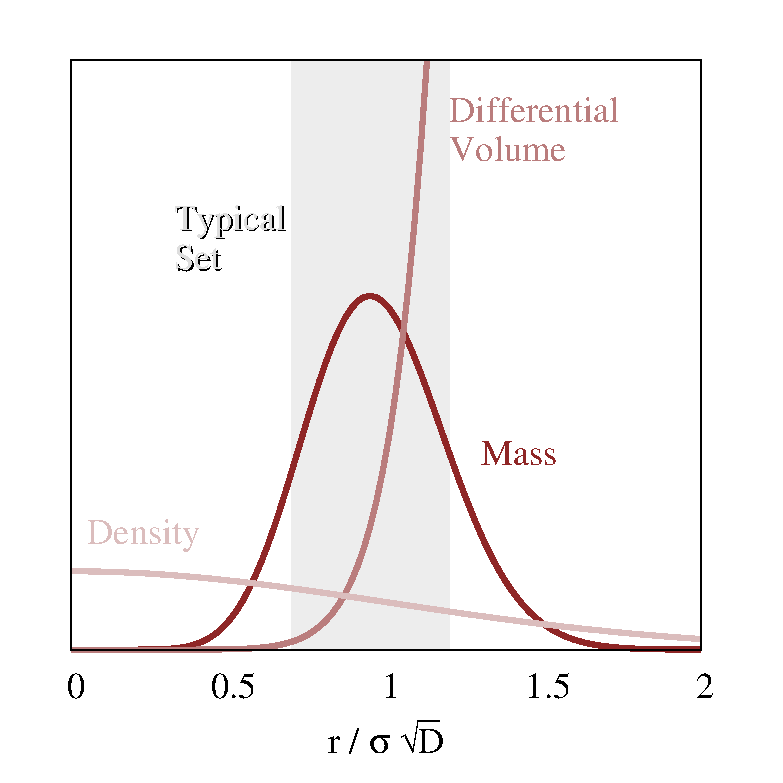
\includegraphics[width=3in]{conc_of_meas_anal.eps}
\caption{In high dimensions real probability distributions generically 
assign almost all of their probability into a singular neighborhood known as
the typical set.  This is apparent even from a probability density function 
representation: although the density concentrates around the corresponding
mode, the volume over which we integrate that density is much larger away
from the mode.  These two opposing trends balance to give the typical set.}
\label{fig:conc_of_meas_anal}
\end{figure*}

Because samples recover all expectations, they too must concentrate 
across the typical set (Figure \ref{fig:samples}).  Consequently, we can also 
use samples to simulate concentration of measure.  For a given $D$ we 
generate a sample from our target probability using a univariate Gaussian 
random number generator available in any computing library,
%
\begin{equation*}
\theta_{d} \sim \mathcal{N} \! \left(0, \sigma^{2} \right),
\end{equation*}
%
and compute the corresponding radial distance 
$r = \sqrt{ \sum_{d = 1}^{D} x_{d}^{2} }$.  Generating a sequence of samples 
and then histogramming the radial distance reveals the same $\chi$ distribution 
that we arrived at analytically (Figure \ref{fig:concentration_of_measure_emp}).

\begin{figure*}
\centering
\begin{tikzpicture}[scale=0.35, thick]
  \draw[-,color=white] (-12, 0) to (12, 0);
  
  \begin{scope}
  \clip (-12, -6) rectangle (12, 10);
  \foreach \i in {0, 0.05,..., 1} {
    \draw[line width={30 * \i}, opacity={exp(-8 * \i)}, dark] 
      (-10, 0) .. controls (-10, 15) and (-5, 5) .. (0, 5)
      .. controls (5, 5) and (10, 8) .. (10, 0)
      .. controls (10, -8) and (5, -3) .. (0, -3)
      .. controls (-5, -3) and (-10, -5) .. (-10, 0);
  }
  
  % Mixing
  \fill[color=dark] (-6, -3) circle (7pt);  
  \fill[color=light] (-6, -3) circle (5pt);
  
  \fill[color=dark] (-4.75, -3.25) circle (7pt);  
  \fill[color=light] (-4.75, -3.25) circle (5pt);
  
  \fill[color=dark] (-3, -3.5) circle (7pt);  
  \fill[color=light] (-3, -3.5) circle (5pt);
  
  \fill[color=dark] (-2, -3.5) circle (7pt);  
  \fill[color=light] (-2, -3.5) circle (5pt);
  
  \fill[color=dark] (-0.3, -3) circle (7pt);  
  \fill[color=light] (-0.3, -3) circle (5pt);  
  
  \fill[color=dark] (0.4, -3.4) circle (7pt);  
  \fill[color=light] (0.4, -3.4) circle (5pt);
  
  \fill[color=dark] (2.9, -3.2) circle (7pt);  
  \fill[color=light] (2.9, -3.2) circle (5pt);
  
  \fill[color=dark] (4, -4.1) circle (7pt);  
  \fill[color=light] (4, -4.1) circle (5pt);
  
  \fill[color=dark] (6.5, -4.8) circle (7pt);  
  \fill[color=light] (6.5, -4.8) circle (5pt);
  
  \fill[color=dark] (6.8, -4.7) circle (7pt);  
  \fill[color=light] (6.8, -4.7) circle (5pt);
  
  \fill[color=dark] (8.6, -4.75) circle (7pt);  
  \fill[color=light] (8.6, -4.75) circle (5pt);
  
  \fill[color=dark] (9.65, -2.75) circle (7pt);  
  \fill[color=light] (9.65, -2.75) circle (5pt);
  
  \fill[color=dark] (9.85, -0.8) circle (7pt);  
  \fill[color=light] (9.85, -0.8) circle (5pt);
  
  \fill[color=dark] (10, 0.7) circle (7pt);  
  \fill[color=light] (10, 0.7) circle (5pt);
  
  \fill[color=dark] (9.8, 2.25) circle (7pt);  
  \fill[color=light] (9.8, 2.25) circle (5pt);
  
  \fill[color=dark] (9.6, 3.75) circle (7pt);  
  \fill[color=light] (9.6, 3.75) circle (5pt);
  
  \fill[color=dark] (8.5, 4.75) circle (7pt);  
  \fill[color=light] (8.5, 4.75) circle (5pt);

  \fill[color=dark] (7.3, 5.3) circle (7pt);  
  \fill[color=light] (7.3, 5.3) circle (5pt);
  
  \fill[color=dark] (5.25, 5.45) circle (7pt);  
  \fill[color=light] (5.25, 5.45) circle (5pt);
  
  \fill[color=dark] (5, 5.65) circle (7pt);  
  \fill[color=light] (5, 5.65) circle (5pt);
  
  \fill[color=dark] (2.25, 4.8) circle (7pt);  
  \fill[color=light] (2.25, 4.8) circle (5pt);
  
  \fill[color=dark] (1.5, 5.1) circle (7pt);  
  \fill[color=light] (1.5, 5.1) circle (5pt);
  
  \fill[color=dark] (-0.6, 5) circle (7pt);  
  \fill[color=light] (-0.6, 5) circle (5pt);
  
  \fill[color=dark] (-1.85, 5) circle (7pt);  
  \fill[color=light] (-1.85, 5) circle (5pt);
  
  \fill[color=dark] (-4.25, 6.5) circle (7pt);  
  \fill[color=light] (-4.25, 6.5) circle (5pt);

  \fill[color=dark] (-5.75, 7.4) circle (7pt);  
  \fill[color=light] (-5.75, 7.4) circle (5pt);
  
  \fill[color=dark] (-6.5, 7.5) circle (7pt);  
  \fill[color=light] (-6.5, 7.5) circle (5pt);
  
  \fill[color=dark] (-8.25, 8) circle (7pt);  
  \fill[color=light] (-8.25, 8) circle (5pt);
  
  \fill[color=dark] (-9.2, 7) circle (7pt);  
  \fill[color=light] (-9.2, 7) circle (5pt);
  
  \fill[color=dark] (-9.7, 5.3) circle (7pt);  
  \fill[color=light] (-9.7, 5.3) circle (5pt);
  
  \fill[color=dark] (-10.1, 4) circle (7pt);  
  \fill[color=light] (-10.1, 4) circle (5pt);
  
  \fill[color=dark] (-10, 2.2) circle (7pt);  
  \fill[color=light] (-10, 2.2) circle (5pt);  
  
  \fill[color=dark] (-10.2, 1.4) circle (7pt);  
  \fill[color=light] (-10.2, 1.4) circle (5pt);  

  \fill[color=dark] (-9.9, -0.1) circle (7pt);  
  \fill[color=light] (-9.9, -0.1) circle (5pt);  

  \fill[color=dark] (-9.5, -1.8) circle (7pt);  
  \fill[color=light] (-9.5, -1.8) circle (5pt);  

  \fill[color=dark] (-8.3, -3) circle (7pt);  
  \fill[color=light] (-8.3, -3) circle (5pt);  
  
  \end{scope}
\end{tikzpicture}
\caption{Because samples recover expectations asymptotically,
large sequences of samples must concentrate in the typical set.
This provides a means of visualizing concentration of measure,
and will prove a powerful way to estimate expectations.
}
\label{fig:samples}
\end{figure*}

\begin{figure*}
\centering
\subfigure[]{ 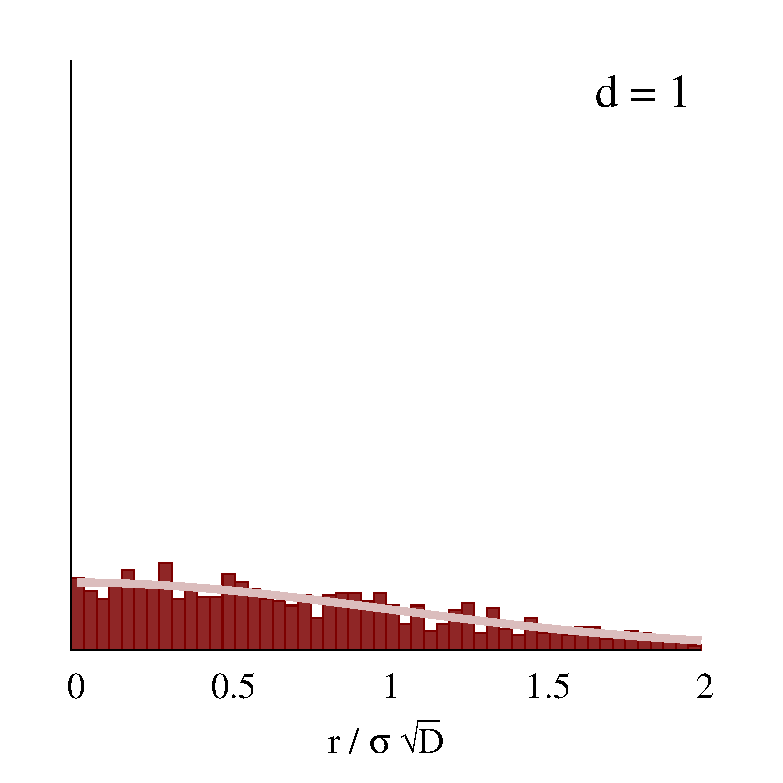
\includegraphics[width=1.85in]{gauss_hist1.eps} }
\subfigure[]{ 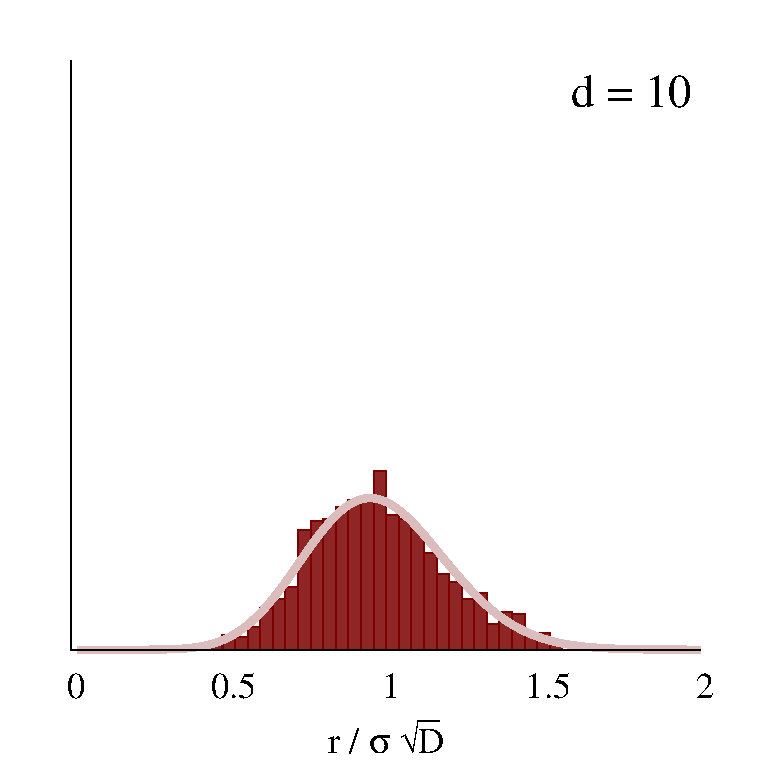
\includegraphics[width=1.85in]{gauss_hist2.eps} }
\subfigure[]{ 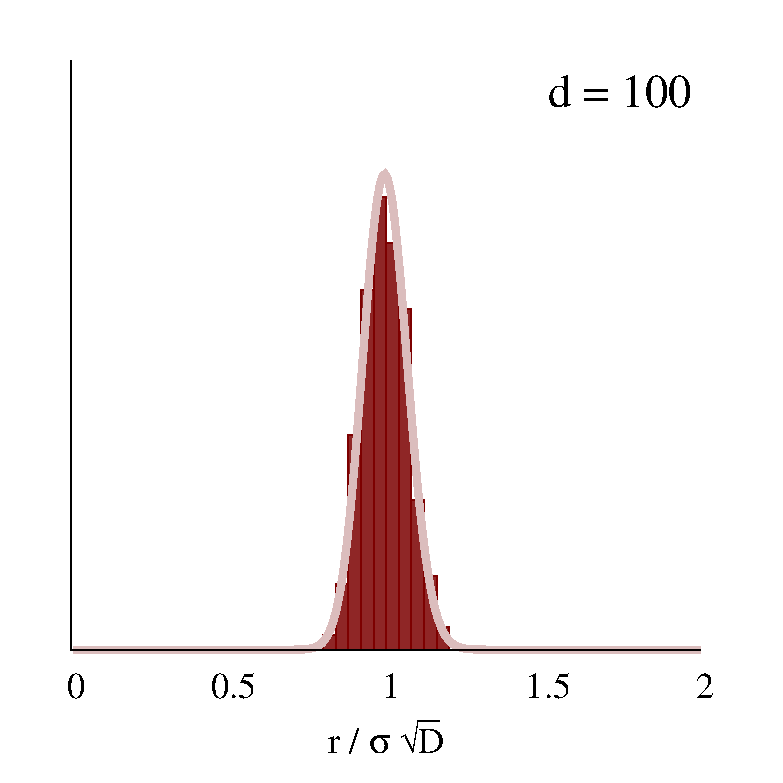
\includegraphics[width=1.85in]{gauss_hist3.eps} }
\caption{Concentration of measure can be visualized with samples 
from a given distribution, which concentrate across the typical set.  
For low-dimensions the concentration is weak and the typical set 
is diffuse, but as the dimensionality of the target distribution grows
so too does the concentration of measure.
}
\label{fig:concentration_of_measure_emp}
\end{figure*}
